\section{Results}
\label{sec:results}

The primary experiment is the Class~A search for a drifting, unresolved
spectral carrier: \NWinA{} fine-channel windows toward \NSysClassA{}
systems. The Class~B search for an unresolved spectral excess is secondary
and carries no drift discrimination: \NWinB{} coarse windows. Together they
are the \NWindows{} windows of the primary census. \textbf{No event
satisfied the confirmation criterion set out in \S\ref{sec:summary}.} What
follows is first how deep the search reaches, and then what it found and how
each finding was disposed of.

\subsection{Sensitivity: the power at which a carrier would have been
found} \label{sec:pninetysel}

\emph{The sensitivity of this survey is a recovery completeness of one epoch,
and not a threshold.} Artificial carriers were injected at a random
sub-channel phase and a random drift from each window's own grid and recovered
through the unchanged pipeline; the power at which nine in ten come back is
$\mathrm{EIRP}_{90}$, the only sensitivity quoted here, measured through the
single-epoch trigger and the localisation at the stellar position inside one
execution block. \textbf{It is therefore the power at which a
carrier would have produced a crossing and not the power at which one would
have been confirmed}, because confirmation needs a second and separated epoch,
which the archive supplies for some systems and not others whatever their
depth (\S\ref{sec:confirmability}). The \NCtrl-position spatial rank decides
nothing and is not charged against it either: charging it would cost a further
factor $\SensCostLike$ and in \SensNRingHiUnres{} bright-ring windows could not
be met at any injected power (Fig.~\ref{fig:strata}).

\emph{Measured that way the completeness is one number for the class.} Nine
carriers in ten are recovered at $\EirpNinetyMultA\,P_{\rm trig}$; the sampling
error of that pooled value is $\pm\SensBootPct$ per cent, which is a statement
about the class average and about no individual window. It is a total power
set against a nominal threshold: $P_{\rm trig}$ is the bare
$\LtCommonSnr\sigma$ of the window itself, and the loss a channel-confined
carrier suffers to the correlator's spectral response is carried by the
injected tones, so it sits inside the measured factor --- $\times\RpRespFac$
of it --- and is not applied to the result as well
(Appendix~\ref{app:conventions}). Every one of the
\SensNInj{} directly injected Class~A windows resolves a ninety per cent point
of its own, and the value does not depend on the brightness of its control
ring: the \SensNRingHi{} windows whose ring carries resolved emission come
back at $\SensRingHi\,P_{\rm trig}$ against $\SensRingLo$ for the rest
(Fig.~\ref{fig:strata}). Class~B carries
its own factor $\EirpNinetyMultB\,P_{\rm trig}$, measured the same way from
\SensNToneCoarse{} carriers injected into \SensNInjCoarse{} coarse windows of
\SensNInjCoarseBlock{} execution blocks; it is what sets the limits for
Barnard's Star, Wolf~359 and Proxima.

\emph{The resulting limits.} The median Class~A window reaches
$\EirpNinetyWinMedA$\,W of equivalent isotropic radiated power and the median
system, on its best window, $\EirpNinetySysMedA$\,W, with a spread across
systems of $\EirpNinetySysLoA$--$\EirpNinetySysHiA$\,W
(Fig.~\ref{fig:classasens}a). The round $10^{15}$\,W level is reached for
\NSysEfifteen{} of them. The calibration of the factor is good to
$\times\SensFacLo$--$\times\SensFacHi$ (Table~\ref{tab:p90budget}); that is
the interval on the median and on the counts, and not on any one window's
limit. One bias is not inside it, runs one way only, and is \emph{not}
included in the values quoted here: an injected carrier is
added to already calibrated visibilities and so suffers no atmospheric
decorrelation, whereas a real carrier does. Measured block by block from the
phase rms the observatory records on each block's phase calibrator
\citep[\S10.4.9]{ALMAHandbook}, through the standard phase-scatter relation
\citep[Eq.~3]{Richards2022}, it leaves the median limit optimistic by
\SensDecorPct{} per cent and the median window above \SensDecorHiGHz{}\,GHz by
\SensDecorHiPct{} per cent, so the limits at the top of the frequency range
are the least secure quoted here. \textbf{The \RpDecNUn{} blocks whose
delivery exposes no such record are not a random subset of the
\SensDecorNBlkTot}: their longest baseline has a median of \RpDecBlUn\,m
against \RpDecBlMeas{} for the \SensDecorNBlk{} that do, and it is the long
baselines that lose coherence. Matching each of their windows to the measured
blocks within a factor of two in baseline length puts the correction at
\RpDecMatchMed{} per cent in the median and \RpDecMatchHi{} at the ninetieth
percentile, so their limits are conditional on a calibration performance the
archive does not report.

\emph{Two further losses act window by window, and both are divided out of
the limits above rather than quoted beside them}
(Appendix~\ref{app:conventions}). The search's phase centre omits the annual
parallax, which displaces the star by at most \SensBeamsMax{} of a synthesised
beam and makes the median Class~A limit shallower by \PxaShiftWinPct{} per
cent, while \PxaMissingStar{} in \PxaMissingEb{} has no astrometric keys and
is left uncorrected. That correction is concentrated rather than general,
which is why the median limit moves far more than the median window's own
factor (Table~\ref{tab:p90budget}): \RpPxNNone{} of the \NWinA{} windows need
none at all, while \RpPxNBig{} lose more than a tenth and lie around the
middle of the distribution of limits. The second
loss the injections do not reproduce at all, each carrier being laid down at
one frequency per integration while a real one sweeps within it.
\textbf{It costs nothing in the median window and up to $\times\SmcFacWorst$
in the \SmcNAbove{} finest-channel ones, which are also the deepest}: the best
Class~A window moves from $\SmcWinLoWas$ to $\EirpNinetyWinLoA$\,W, and
\SmcLostStars{} drops out of the \SmcSysEfifteenWas{} systems that would
otherwise reach $10^{15}$\,W.

\emph{Carriers were injected directly into \SensNInj{} of the \NWinA{}
Class~A windows, \SensNInjPct{} per cent, and the result transferred to the
remaining \SensNTransfer, which is the dominant caveat on all of the above.}
The injected windows are the Class~A windows of execution blocks drawn in a
stratified random order fixed in advance and without reference to which
windows hold a crossing; they hold \SensNCrossAch{} crossings against the
\SensNCrossExp{} the population rate predicts. \emph{The unit is the block and
not the window}, because a block's calibrated visibilities are what an
injection campaign has to rebuild, so band and array were fixed by the draw
and the conditions that vary within a block were compared with the population
afterwards. \textbf{That comparison covers \RpNAxis{} properties} --- channel
width, integration time, noise, control-ring brightness, the channels a
carrier at the drift ceiling crosses in one track, and the intra-integration
retention --- and on every one the injected windows span the central
eight-tenths of the population, five agreeing in the median to
\RpCovOtherPct{} per cent. The sixth, \RpCovWorstAxis, does not: the injected
windows are $\times\RpCovWorstRatio$ noisier, which follows from drawing whole
blocks, and it is also the property the measurement is built to be
insensitive to, each ladder being in units of its own window's threshold.
That is measured rather than assumed: splitting the injected set at the median
of each property in turn moves the ninety per cent point by at most
\RpFacShiftMax\,$P_{\rm trig}$. The draw controlled the array, but the
achieved mix still departs from the population by \SensCovWorstPct{} per cent
of the sample; re-weighting the pooled curve by the survey's own composition
gives
$\SensPooledArrWeighted\,P_{\rm trig}$ against the adopted
$\EirpNinetyMultA$.

\textbf{A window that was not injected therefore carries an estimated
$\mathrm{EIRP}_{90}$}, and across the injected windows the ninety per cent
point ranges from $\times\SensIndivFacLo$ to $\times\SensIndivFacHi$ of the
adopted factor: that dispersion, not the calibration interval above, is what
one uninjected window's own limit is uncertain by. Because a system's limit is
its best window, a minimum over several such estimates could favour windows
whose own factor falls below the class average; drawing each window's factor
from the \SensNInj{} measured ones instead, over \ScRsNTrial{} trials, moves
the per-system median deeper by \ScRsMedShiftPct{} per cent, holds the count
at $10^{15}$\,W to \ScRsNLo--\ScRsNHi{} in nine trials in ten and spreads one
system's own limit by $-\ScRsSysLoPct$ to $+\ScRsSysHiPct$ per cent, so the
estimate is mildly conservative. But \textbf{the best window was itself injected into for only
\SmcNMeasSys{} of the \NSysClassA{} systems}: for the other \SmcNEstSys{} the
headline limit is an estimate.

\emph{A carrier that is not always radiating is penalised in proportion.} The
de-drifted stack is coherent across a whole execution block, so over
\DutyNTrial{} trials at duty cycles down to \DutyCycleMinPct{} per cent the
recovered amplitude followed the duty cycle to \DutyAttenDevPct{} per cent: a
transmitter radiating a tenth of the time needs $\DutyPowFac\times$ the power
quoted above. Those trials carry no drift, so the joint drifting and
intermittent case is not measured here.

\begin{table}
\centering
\scriptsize
\caption{What sets $\mathrm{EIRP}_{90}$, and in which direction. The
uncertainty on the calibration is an uncertainty on the class-average factor,
and so on any statistic formed over many windows; its flux term is
band-dependent, so the submillimetre windows carry the larger combined
figure. The spread between windows
is an observed dispersion and is the statement about one window's own limit;
the signed terms are biases, stated with their direction rather than folded
into an error bar, and the decorrelation term is measured in \SensDecorNBlk{}
of the \SensDecorNBlkTot{} blocks and not imputed to the rest.}
\label{tab:p90budget}
\tiny
\setlength{\tabcolsep}{2pt}
% GENERATED by sens_r11.py -- do not hand-edit.
\begin{tabular}{@{}l@{~~}r@{~~}>{\raggedright\arraybackslash}p{0.37\columnwidth}@{}}
\hline
 & value & what it does to the limit \\
\hline
Class-average completeness & $\times3.03$ & nine carriers in ten recovered at this multiple of a window's own trigger power. \emph{Measured} in the 49 Class~A windows injected directly and \emph{estimated}, at this factor, in the other 353 \\
\hline
\multicolumn{3}{@{}l}{\emph{Uncertainty on that calibration} (per cent), combined in quadrature} \\
The factor itself & $\pm2$ & sampling error of the pooled value over the 49 injected windows \\
Absolute flux scale & $\pm\BudFlux$ & the observatory's own band-dependent specification (\BudFluxSource): \BudFluxSpec, weighted over this sample's bands \\
Distance and visibility scale & $\pm\BudDistVis$ & the Gaia parallaxes, which enter as $d^{2}$, and the block-to-block visibility scale \\
\emph{Combined} & $-11/+11$ & $\times0.89$--$\times1.11$ on the factor, and so on the median limit and on the system counts; $\pm\BudCombWorst$ for the \BudNHiWin{} Class~A windows in \BudHiBandWord~\BudHiBands, at \BudHiGHzList\,GHz \\
\hline
\multicolumn{3}{@{}l}{\emph{Spread between windows}. An observed dispersion, not an error bar.} \\
Window to window & $\times0.80$--$\times1.58$ & the 49 injected windows resolve 2.41--4.80\,$P_{\rm trig}$ individually. This, and not the interval above, is what an estimated limit is uncertain by; it is wider, and it applies to \SmcNEstSys{} of the \NSysClassA{} systems \\
\hline
\multicolumn{3}{@{}l}{\emph{Applied}. Folded into every limit quoted, and so not combined with the above.} \\
Intra-integration smearing & $\times1.00$--$\times\SmcFacWorst$ & a carrier sweeps through part of a channel within one integration and the injected ones do not: $\eta_{\rm smear}$ at the drift that sets a ninety per cent point, from each window's own integration length where it is recorded (\SmcNMeas{} windows) and from the longest delivered anywhere where it is not (\SmcNBound) \\
Annual parallax & $\times1.00$--$\times2.06$ & the phase centre omits it, so each limit is divided by the amplitude a compact source retains at its own displacement, a median \PxaLossMedPct\,per cent \\
\hline
\multicolumn{3}{@{}l}{\emph{Signed terms}. A bias is not an error bar and is not added to one.} \\
Channel response & $\times\RpRespFac$ & the share of a channel-confined carrier the peak channel keeps. Carried by the injections, so already inside the completeness above, which is this factor times a margin of $\times\RpMarginNinety$ over the nominal trigger \\
\quad its residual & $+\InjShortPct$ & the injected profile falls short of the exact response: \emph{conservative} \\
Decorrelation & $+0/+\SensDecorPct$ & measured block by block from the phase rms the observatory records on each block's phase calibrator, which an injected carrier does not suffer and a real one does: $+\SensDecorHiPct$ above \SensDecorHiGHz\,GHz, and more than $+\SensDecorTailLevelPct$ in \SensDecorTailPct{} per cent of windows \\
\hline
\end{tabular}

\end{table}

\begin{figure}
\centering
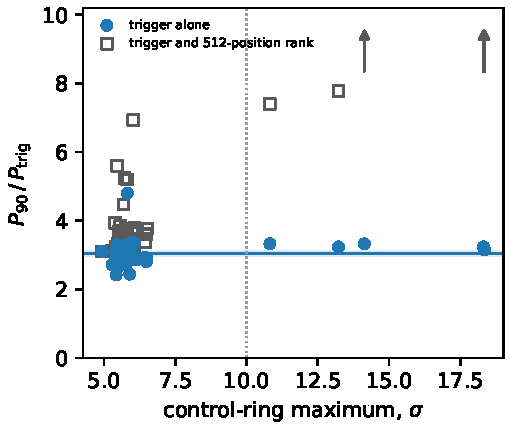
\includegraphics[width=0.96\columnwidth]{figures/sens_ring.pdf}
\caption{Why one completeness factor serves the whole class. Each of the
\SensNInj{} of the \NWinA{} Class~A windows injected directly is plotted at
the power that recovers nine carriers in ten, against the maximum of its own
\NCtrl-position control ring. Filled circles are the criterion adopted
here --- the trigger and localisation at the star --- with the pooled value
and its uncertainty as the line and band; they show no trend with the ring.
Open squares add the demand that the carrier outrank every control position,
and arrows mark the windows that then reach ninety per cent at no injected
power. Dotted, the $\SensRingRule\sigma$ ring brightness above which a ring
carries resolved emission rather than noise.}
\label{fig:strata}
\end{figure}

\begin{figure*}
\centering
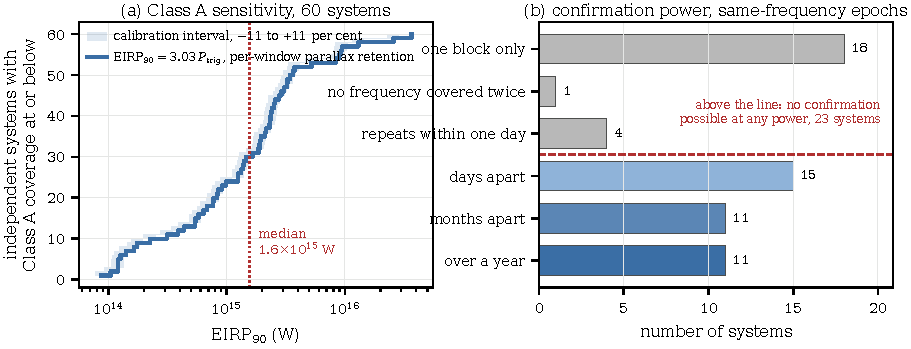
\includegraphics[width=0.92\textwidth]{figures/classa_sensitivity.pdf}
\caption{\textbf{The two completenesses of the carrier search, over the same
\NSysClassA{} systems.} \emph{(a)}~Single-epoch trigger completeness: the
cumulative number of systems whose best window reaches a given
$\mathrm{EIRP}_{90}$ (Table~\ref{tab:quantities}), evaluated as
$\EirpNinetyMultA\,P_{\rm trig}$ with each window's own annual-parallax
retention applied; the shaded band is the calibration interval of
Table~\ref{tab:p90budget}. \emph{(b)}~Confirmation completeness, which no
amount of power buys: systems grouped by the longest separation between two
execution blocks covering a common frequency, more than \EpSep{} day counting
as independent. \textbf{Left of the dashed line, \RcNoRepSys{} systems have no
such pair, and for them confirmation was not possible at any sensitivity in
panel~(a)}: what panel~(a) gives them is a crossing limit, not a detection
limit.}
\label{fig:classasens}
\end{figure*}

\subsection{The nearest stars: Barnard's Star and Wolf~359}
\label{sec:barnardswolf}

Barnard's Star is the second-nearest stellar system and Wolf~359 the third if
brown dwarfs are excluded, and to our knowledge these are the first millimetre
or submillimetre technosignature limits for either \citep{Enriquez2017,
Price2020, Margot2023}. Both are non-detections. \emph{Both limits come from
the secondary Class~B experiment and not from the carrier search}: the archive
holds only coarse Band~6 windows toward these stars, so what is constrained is
an unresolved spectral excess and not a drifting carrier. On the
$\mathrm{EIRP}_{90}$ convention of \S\ref{sec:pninetysel} Barnard's Star
reaches $\EirpNinetyBarnLo$--$\EirpNinetyBarnHi$\,W over \NWinBarn{} windows
and Wolf~359 $\EirpNinetyWolfLo$--$\EirpNinetyWolfHi$\,W over \NWinWolf.

\subsection{Threshold crossings and how each was disposed of}
\label{sec:technosearch}

\emph{The result is a chain of three tests, and it is read in one direction.}
Of the windows the search covers --- the \NWindows{} of the primary census
and the archival-tail blocks beside them --- \EvNCrossRaw{} hold a cell
reaching $T\geq5$ at the stellar position. \EvNCrossFlag{} lie in the one
execution block that fails the quality criterion of \S\ref{sec:bdblock}, fixed
before it was applied, so the population that characterises the search is the
\EvNCrossQp{} in quality-passing data and those \EvNCrossFlag{} are reported
beside it. The molecular-line mask, $\pm\MaskHalfKms$\,km\,s$^{-1}$ wide in
each star's own rest frame, places \MkNCoinc{} of the \EvNCrossQp{} within
that distance of a catalogued transition; \MkNSODecideWord{} of those
coincidences are with a species no debris disc has been shown to carry and are
reported rather than acted on (Appendix~\ref{app:linemask}), leaving
\EvNAttrQp{} attributed and \EvNUnattrQp{} unattributed. The attributions are
kinematic and not an accident of bandwidth: in the delivered frame,
\AppMTubeObs{} of the
\AppMNCrossF{} crossings with a measured peak frequency fall within
$\pm\DispoHalfKms$\,km\,s$^{-1}$ of a transition these setups were tuned to, against
\AppMTubeNull{} expected were each peak free to land anywhere on its own
window's grid (Appendix~\ref{app:rfi}). Of the unattributed,
\EvNRankQp{} outrank all \NCtrl{} control positions of their own window, and
none was found again in any later epoch covering its frequency. \textbf{No
crossing survives the chain, and this survey reports no detection.}
Figure~\ref{fig:chain} counts what survives each step and
Tables~\ref{tab:ledger} and~\ref{tab:ledgercont} list every crossing.

\emph{Anything bright in a window hides a weaker carrier behind it, so the
weaker cells were sought too.} The de-drifted statistic is retained in every
channel, so behind a window's tabulated crossing --- its largest cell ---
weaker above-trigger cells can be read as well, neighbouring channels counting
as one. Re-read that way, the
\CkNWin{} of the \NWinA{} Class~A windows that retain such a profile --- the
other \CkNWinNotCov{} retain none --- hold \CkNPrimary{} maxima at or above
the trigger and \CkNSecondaryWord{} weaker cells besides,
in \CkNSecWin{} windows and as many as
\CkNSecMax{} in one. \CkNSecAttr{} are the resolved carbon monoxide of a disc
spread over channels; the \CkNSecUnattrWord{} unattributed ones, toward
\CkSecStars, each have \CkCovLo--\CkCovHi{} covering blocks and
\CkNRecurWord{} reaches the trigger in any of them, the deepest repeat being
$T_\star=\CkTrepHi$. Applied to the window maxima the
rule returns \CkRegN{} of the \EvNCrossRaw{} tabulated crossings to
\CkRegDev{} of a channel; the \CkRegMiss{} it misses are the \EvNCrossFlag{}
of the failing block, whose repaired profile was not retained, and crossings
whose own window retains no usable profile.
Cells are counted in the controls too, and outside the mask the star holds
\CkRatioLo--\CkRatioHi{} times as many as a control position at every level
from $T=\CkLadderLo$ to the trigger, with no step where a carrier search would
put one; the expectation that follows is \S\ref{sec:trigunif}'s.

\subsubsection{Most of the crossings are expected by chance}
\label{sec:trigunif}

The trigger is a threshold on a statistic and not a false-alarm rate: the
number of searched channel\,$\times$\,drift cells per window spans
\TuCellsDecades{} decades, so one level buys very unequal protection. How
many crossings chance should produce is therefore measured window by window,
over the \CeNWin{} Class~A windows of the census and with one condition on
both sides of the comparison: a cell at the stellar position that reaches the
trigger and that the line mask does not attribute. A window's own \NCtrl{}
control positions measure how often a position in that field reaches the
trigger, and the window's own channel grid measures how often such a position
would fall inside an attribution window, which takes \CeMaskPct{} per cent of
the total. The control positions differ from the star in one respect that
bears on this: they carry no continuum, so a calibration error that varied
with frequency would raise the star and not them. Measured on the continuum
these stars are found to have, the windows where such an error could reach
the trigger hold no crossing and bound it below \CxResidHiPct{} per cent
(Appendix~\ref{app:radius}). Chance predicts \CeExp{} unattributed Class~A
crossings, with \CeLo--\CeHi{} allowed by resampling the execution blocks the
windows come from, and \CeObs{} are found. Counting cells rather than windows
on both sides moves the two together: the same \CkNCtrlPos{} control positions
predict \CkExp{} cells, \CkExpSec{} of them beside a window's largest, against
\CkNObs{} and \CkNSecUnattr{} found and \CkLo--\CkHi{} allowed, because a
control position holds a second above-trigger cell about as often as a star
does (\S\ref{sec:technosearch}). A further \CeNTailCrossWord{} unattributed
crossings, both toward \CeTailStar, lie in archival-tail blocks the catalogue
does not tabulate window by window, and enter neither side.

The expectation is a sum of rates measured at control positions, and the
reserved blocks measure how far a star departs from them: carrying that
difference through moves it to \CeExpX, and the count agrees with chance
either way. The width of the range allowed is what the comparison can say and
no more --- an added population of as many as \CeAddBlind{} crossings would
sit inside it unremarked. What tests each crossing individually is the
recurrence test of \S\ref{sec:etacrv}.

\subsubsection{One execution block accounts for four of the crossings}
\label{sec:bdblock}

\BdNCross{} crossings belong to \BdStar{} (\BdAlias), all in one ACA execution
block, \texttt{\BdBlock}, whose whole field is above threshold:
\BdNCtrlAbove{} of \BdNCtrl{} control positions exceed $T=5$, where the median
of a window's own control ensemble is \BdSurvCtrlMed{} across the survey. Its single-integration noise is as
predicted (\BdRmsMeas\,Jy against \BdRmsPred\,Jy) but does not integrate down
--- a jackknife on the channel mean gives \BdJack\,Jy against
\BdThermal\,Jy thermal --- so a slow drift common to every channel and
position inflates the statistic across the field, while the \BdNSibling{}
sibling executions of the same field, array and setup reach only
$T_\star=\BdSibTMax{}$ and produce no crossing. \emph{What is inflated is the
field and not the star:} the strongest of the four reaches
$T_\star=\EvFlagTStarHi$ where its own controls peak at \EvFlagCtrlAtHi, and
\EvFlagNgeLo--\EvFlagNgeHi{} of the \BdNCtrl{} stand above the star. The
criterion fails this block and no other
(Appendix~\ref{sec:blockquality}), so its \BdNCross{} crossings are reported
apart from the \EvNCrossQp{}; Appendix~\ref{app:rfi} carries what the block
might instead be.

\subsubsection{Stellar flares are excluded by a broadband prediction}

The sample contains known flare stars. But a millimetre flare raises every
channel of a window alike, so one able to produce a single-channel crossing at
the trigger must produce a $5\sqrt{N}\sigma$ continuum event in the same
integrations. Over the \FlNCont{} crossings with a recoverable continuum
measurement that prediction runs \FlPredLo--\FlPredHi$\sigma$, against an
observed continuum statistic of median \FlObsMed{} with $|Z|<3$ in \FlNQuiet{}
of them. One block settles it: \FlEgStar{} \texttt{\FlEgEb} holds both a
crossing ($T_\star=\FlEgT$) and the millimetre flare of
\citet{MacGregor2020}, and \emph{that flare contributes \FlEgContrib$\sigma$
to the single-channel statistic} --- raising the continuum at $Z=\FlEgContZ$
while the crossing's own de-drifted track reaches $Z_{\max}=\FlEgTrackZ$.

\subsection{$\beta$~Pictoris: an astrophysical positive control, and the
obstacle it identifies} \label{sec:bpicval}

\emph{A search that finds nothing must show that it could have found
something, and the survey's strongest features show exactly that.} The
frozen pipeline recovers the $\beta$~Pictoris circumstellar carbon monoxide
blind, without being told the disc is there. It recovers it in two
rotational transitions and in \CsBpCoBlocks{} independent execution
blocks spanning \BpBaselineYr\,yr, and in \NStageOneBpicEb{} of those the
star also outranks every control: \BpicNFlagThree{} Band~3 windows at
$T_\star$ up to \BpicBThreeTsym, and \BpicNFlagSix{} Band~6 windows at
\BpicBSixTsym. The identification is kinematic and does not rest on those
statistics. Carried through the frame chain --- to the barycentre at each
block's own epoch, then to the star's rest frame --- all \BpicPanelNCo{}
crossings lie within \BpicDvCoHi\,km\,s$^{-1}$ of the stellar systemic
velocity, in the two lowest CO transitions of a star with mapped
circumstellar CO \citep{Dent2014,Matra2017}. The Band~3 peaks agree across blocks to
\BpRecThreeTuneChanMax{} channel once each block's own tuning is removed, so
any apparent drift is far below the grid searched. The alternative reading
requires a transmitter placed by coincidence at matched offsets from two CO
transitions of one star.

It is also the control that shows the recurrence test of
\S\ref{sec:etacrv} working in the positive direction: every flagged
$\beta$~Pictoris carbon-monoxide feature is recovered in an independent
execution block, the screened Band~6 window returning
$T_\star=\BpRecTTwo{}$ in the second block of its own recurrence set. A
non-recurrence elsewhere means nothing unless the same machinery recovers a
repeat where one exists.

\emph{One of those blocks is a counterexample, and it is the more useful half
of the control.} In it several of the \NCtrl{} control positions exceed the
stellar statistic, so the spatial rank disfavours a window holding carbon
monoxide known to be real and centred on the star; the disc is resolved on
the scale of the primary beam in that configuration, which is the geometry
the statistic is built to reject. The rank is therefore a test of
compactness and not of authenticity, and on a real extended source it errs
conservatively --- a stronger statement than a clean positive control, because
it bounds the diagnostic's reach as well as demonstrating it
(Fig.~\ref{fig:bpiccontrol}).

%% fig:bpiccontrol MOVED to Appendix B (sections/app_C_spatialnorm.tex),
%% which is the appendix about the spatial statistic this figure bounds.
%% 0.36 pp off the main text; Sec. 5.4 cites it.


HD~48370 is the complementary case and is equally instructive. Its crossing
reaches $T_\star=\HdTsym$, but the control ring rises with the star, to
\HdRingMax, as emission filling the primary beam does. The velocity matches
the prominent CO($2{\to}1$) that \citet{Cataldi2023} report toward the
source and flag as possible foreground cloud emission. The block's
$^{13}$CO($2{\to}1$) window is bright at the ring and faint at the star.
What identifies the extended emission is therefore the \emph{level} of the
control ring and not the star's rank against it --- the star here outranks
every control --- which is why the window-level flag of
Appendix~\ref{sec:blockquality} is defined on the ring's median.

\emph{Taken together, these two results identify the dominant obstacle for
millimetre technosignature searches, and it is not sensitivity.} The
strongest apparent signals in this survey are circumstellar and foreground
molecular emission, and \NAttributed{} of the \NCross{} crossings land on a
catalogued transition. The mask that removes them costs \MkMaskAPct{} per
cent of the Class~A union bandwidth over \FrNSpec{} species, and it is
nevertheless the single most productive test in the chain. The warning for
future work is about line lists rather than about depth, and
Appendix~\ref{app:linemask} puts a number on it.

\subsection{The two crossings that lead their own control fields}
\label{sec:vistest}

Frequencies in this section and the next are in the star's own rest frame,
which is the frame the recurrence test registers in; the delivered ones are in
Table~\ref{tab:cand} and in the ledger.

Two crossings reach a stellar statistic above every one of the \NCtrl{}
control positions in their own window: \EvAStar{} at \RqFreqSx\,GHz and
\EvBStar{} at \RqFreqCp\,GHz, both in Band~\EvABand. Both are tabulated in
Table~\ref{tab:cand}, the first is drawn in Fig.~\ref{fig:event}, and neither
is a detection. The control rank is recorded for them because it says which
crossing was examined first; it disposes of nothing (\S\ref{sec:method}).
\EvBStar's crossing lies $\EvBDv$\,km\,s$^{-1}$ from \EvBLine, a coincidence
reported as a note rather than as a disposition
(Appendix~\ref{app:linemask}). Both events go on to the recurrence test. Each
was also re-fitted in the visibility domain, as \LgNFit{} of the \NCross{}
crossings were, by phase rotating to the star and following the recovered
drift; \LgNLocalCor{} of those fits are consistent with a point source at the
star, and injected sources in the bin these two occupy return
${\rm Re}/\sigma=\RsevReAtFiveMeanA\pm\RsevReAtFiveSdA$, so the fit excludes
none. Its value is that a pedestal fed through a sidelobe from elsewhere in
the field, which a dirty map at the star cannot tell from a source at the
phase centre, is not a point source there. Of the \NCtrl{} control positions
the rank screen uses, \RcNRetCtrl{} retain a dynamic spectrum and
\RcNVisCtrl{} are reachable in the visibilities.

Neither crossing is present when the same stellar-frame frequency is observed
again.
The reading that assumes least is the nearest covering block alone, taken
\RcSxNearH{} and \EvBDeepH\,hours from each discovery: a carrier persisting at
the discovery amplitude would have given $T_{\rm pers}=\RqNearTPersSx$ there
against $\RqNearTRepSx$ measured for \EvAStar{} and $\RqNearTPersCp$ against
$\RqNearTRepCp$ for \EvBStar{} --- whose nearest block is also its deepest ---
ruling out anything above \RqNearFracSx{} and
\RqNearFracCp{} of that amplitude. Over intervals of hours a transmitter
orbiting at 1\,au stays inside the $\pm\RqDispSx$ and
$\pm\RqDispCp$\,km\,s$^{-1}$ half-channel those readings cover, so both
survive an orbit of that period. Combining all \RqNRepSx{} and \RqNRepCp{}
covering blocks deepens the limits to \RcSxFive{} and \RcCpFive{} of that
amplitude, but requires the carrier to hold one channel across baselines of
\RqSpanDSx{} and \RqSpanDCp\,days, over which the same orbit would move it
\RqOrbFarSx{} and \RqOrbFarCp\,km\,s$^{-1}$: those readings constrain only a
carrier stable to half a channel over the whole baseline. At the faintest amplitude consistent with each crossing
having been found at all, the criterion would have recovered a persisting
carrier with probability \RqPowerTrigSx{} and \RqPowerTrigCp: for \EvBStar{}
the silence is not an exclusion, and is not read as one.
Appendix~\ref{app:radius} follows \EvBStar's crossing through every step
of the chain.


\subsection{Recurrence, applied to every unattributed crossing}
\label{sec:etacrv}

A carrier that stays inside the repeat window and radiates through both
observations must be there when the same frequency is observed again. That is
the confirmation criterion, applied in the star's own frame: the predicted
channel follows from the Earth's motion at the repeat epoch and the star's
systemic velocity, the discovery drift is carried to it, and the statistic is
read there, maximised over nothing. The frame matters, because for $\eta$~Crv
it moves the predicted channel by \VnEcrDchan{} channels. A \emph{confirmed
signal} is an \emph{unattributed} crossing that satisfies the criterion
(Table~\ref{tab:quantities}); a line-coincident crossing that satisfies it is
a recurring molecular line, and is reported as one.

None of the unattributed crossings recurred, while \MkAttrRecur{} crossings
attributed to circumstellar or foreground carbon monoxide do recur, as
expected. Those \MkAttrRecur{} are the positive control of this stage and they
test it on both of the ways real emission arises here: \RqNRecurDisc{} are the
resolved circumstellar disc of \RqRecurDiscStars{} and \RqNRecurCloud{} are
foreground gas toward \RqRecurCloudStars, whose sightline carries catalogued
cloud emission at the crossing's own velocity in the local standard of rest
(Appendix~\ref{app:linemask}). No exclusion is formed for them, because what
one would exclude has just been observed. Close to the trigger the control is
thinner than that count suggests: every circumstellar recovery has
$T_\star\ge\RqRecurDiscTLo$, and the \RqNearTrigN{} attributed crossings that
are not recovered are the two faintest tested, both at
$T_\star=\RqNearTrigT$, so there the stage is controlled by
\RqRecurCloudStars{} alone --- by foreground gas rather than by a point
source. All \RcNTested{} unattributed crossings were tested, over
\RcNRepeatMeas{} readings in \RcNRepeatBlock{} execution blocks, and at the
predicted cell the largest statistic over all of them is $\RcTRepMax$ at the
carried drift and \RcTMax{} over every drift trial, against a trigger of 5.

Every exclusion is conditional on a requirement of frequency stability, and it
is a narrow one. The reading is taken at one cell at one drift, so it
constrains only a carrier whose stellar-frame frequency moved by less than
half that cell between the epochs compared: \TjChanKHz\,kHz, which is
$\pm\RqDvLo$ to $\pm\RqDvHi$\,km\,s$^{-1}$ across the \RqNUnit{} crossings
that carry an exclusion, median $\pm\RqDvMed$. A transmitter in a circular
orbit at 1\,au accelerates along the line of sight by up to
\RqOrbAu\,mm\,s$^{-2}$, which keeps it inside that interval for \RqNOrbNear{}
of the \RqNUnit{} over the interval to the nearest covering block and for
\RqNOrbFar{} of them over the longest baseline; at the \WdAGrid\,m\,s$^{-2}$
the drift grid reaches, \RqOrbGridWord{} of the exclusions survive. The search
accommodates planetary acceleration and this test does not, so the two bear on
different classes of transmitter: non-recurrence excludes a carrier that holds
its frequency within those limits and radiates through both observations, and
says nothing at all about one whose orbital motion carries it out of the cell.
That is why the whole window is searched at every drift of the grid at each
repeat epoch, which spans that excursion for \WdNOrbSpan{} of the
\WdNOrbTot{} crossings another block covers.

The amplitude each exclusion reaches is the fraction of the discovery
amplitude still excluded at the trigger, $(T_{\rm rep}+5)/T_{\rm pers}$. Of
the \RcNTested{} crossings tested, \RcNExcl{} carry a quoted exclusion;
\RcNWithheld{} take their discovery amplitude from the block that fails the
quality criterion of \S\ref{sec:bdblock} and \RcNNoSpec{} retains no discovery
spectrum, so none can be formed for those. Over the \RcNExcl{} the repeat
coverage rules out a carrier at a median \RcFracMed{} of the discovery
amplitude and the deepest at \RcFracMin{} of it, but the individual limits run
to \RcFracMax, and for \RcNFracWeak{} of them --- \RcFracWeakList{} --- nothing
below \RcFracWeakLo{} is ruled out. Combining every covering block buys most
of that, and requires the carrier to return to the same cell at the start of
each: the nearest block alone rules out a median \TjFracNearMed{} of the
discovery amplitude, and \TjNNearWeak{} of the \TjCombNCross{} rule out
nothing. The chance that a carrier would have satisfied the criterion is
evaluated at the trigger amplitude $5S/T_\star$ rather than at the
discovery amplitude, which is selected as the largest of many cells at a
statistic of about five and is biased high (Appendix~\ref{app:radius}): it
exceeds \RcPowerLevel{} per cent for \RqNPowerHi{} of the \RcNExcl{} and for
the remaining \RcNPowerLoTrig{} it is \RqLowList. Those \RcNPowerLoTrig{} are
untested rather than excluded. These are conditional detection probabilities
under the persistent-carrier model adopted here, not probabilities that a
candidate was noise: a crossing that does not recur has not been shown to be
anything else.

The \WdNExc{} repeat windows that do hold something above the trigger are
themselves crossings, so a carrier present again would appear in its repeat
block as one; their number agrees with the \WdExpect{} chance predicts in
trials of that size, but each pair must still be asked whether one transmitter
could have produced both members. Table~\ref{tab:pairs} asks it of all
\TjNPair{} pairs, across
\TjNStarPair{} stars, whose two crossings lie within
\WdHalfKms\,km\,s$^{-1}$ of each other in one star's frame. Both fitted drifts are
carried into that frame first, by removing the observatory's own
line-of-sight acceleration: at most \TjFrameMaxHzS\,Hz\,s$^{-1}$ here, but
diurnal, so extrapolating it across days would add an excursion that is not
there.

Two criteria follow, and they partition the pairs differently. Where the drift
grid resolves the interval --- \TjNPower{} of the \TjNPair{} pairs --- the
elapsed time and the two drifts fix the offset a carrier at constant
line-of-sight acceleration would show, and all \TjNPower{} fail that
comparison, by \TjSigMin{} standard deviations in the mildest case. The weaker
demand is any trajectory whose drift stays inside the searched grid and whose
curvature is bounded by the same acceleration ceiling, and it is the one each
verdict rests on: it excludes \TjNExcl{} pairs ---
\TjNExclGrid{} needing a mean drift the search never covered and
\TjNExclTau{} needing an acceleration reversal \TjRatioLo{} to \TjRatioHi{}
times faster than the \TjTauOrbH\,hour quarter period the ceiling allows ---
and leaves \TjNOpen{} not separable, among them \TjNPowerOpen{} of the
\TjNPower{} that the constant-acceleration comparison resolves.
$\beta$~Pictoris is judged by the same criterion. Its two crossings sit at
\TjBpNuLo{} and \TjBpNuHi\,GHz in blocks \TjBpDtH\,hours apart,
\TjBpDvKms\,km\,s$^{-1}$ apart, and both fitted drifts are negative,
$\TjBpDriftLo$ and $\TjBpDriftHi$\,Hz\,s$^{-1}$, so a single carrier would have
had to rise in frequency between the epochs; that needs a mean line-of-sight
acceleration of \TjBpAccelReq\,m\,s$^{-2}$, inside the
\WdAGrid\,m\,s$^{-2}$ ceiling, so the sign settles nothing on its own. The
reversal does: the pair requires one in \TjBpTauH\,hours, \TjBpRatio{} times
faster than the ceiling permits, which is the narrowest margin of the
\TjNExcl{} exclusions and the only one inside a factor of two. The same test
accepts the one pair that is a single emitter, the \TjCtlLine{} line of
\TjCtlStar{} recovered at one stellar-frame frequency \TjCtlDtD{} days apart,
\TjCtlNSig{} standard deviations from the prediction. For the \TjNOpen{} pairs
it cannot
separate, \TjDtOpenMinD{} days to nearly two years apart, nothing measurable
tells one carrier from two, and only the agreement of their number with
chance bears on them.

The \MkAttrExcl{} attributed crossings of the \MkAttrTested{} tested that are
not recovered both remain consistent with their attribution. \RqHrStar's
crossing at \RqHrFreq\,GHz is \RqHrDv\,km\,s$^{-1}$ from CO($2$--$1$) and is
bounded at $T_{\rm rep}<\RqHrTRep$ against the $T_{\rm pers}=\RqHrTPers$ real
carbon monoxide at the discovery flux would have given, a disagreement of only
\RqHrExcl$\sigma$ once that window's noise is measured over the
\RqHrOnsMin{} minutes it integrates, \RqHrRms\,mJy, where its sibling blocks
also lie. \RqAjStar{} is a
serendipitous field star with no measured systemic velocity, so its frame is
the \RqAjFrame{} one; its crossing at \RqAjFreq\,GHz is \RqAjDv\,km\,s$^{-1}$
from the same transition and the bound there is $T_{\rm rep}<\RqAjTRep$
against $T_{\rm pers}=\RqAjTPers$, or \RqAjExcl$\sigma$. Its attribution rests
on a velocity rather than on this test: the sightline carries catalogued
foreground emission at \LsLupVco\,km\,s$^{-1}$ in the local standard of rest,
\LsLupDv\,km\,s$^{-1}$ from the crossing's own velocity in that frame
(Appendix~\ref{app:linemask}). What its repeat blocks show is where that gas
lies rather than whether it can be recovered. All \RqAjNRep{} were taken in
the same \RqAjArray{} configuration with synthesised beams of \RqAjBeamLo{} to
\RqAjBeamHi{} arcsec, so an extended cloud is recovered alike in each, and in
every one the control ring reaches \RqAjCtrlLo{} to \RqAjCtrlHi{} while the
phase centre reads \RqAjStarLo{} to \RqAjStarHi{} with \RqAjNgeLo{} to
\RqAjNgeHi{} of the \NCtrl{} control positions above it: the gas is bright and
it is not at the phase centre. Toward \RqRecurCloudStars{} it is, and over the
\RqCtlNBlock{} covering blocks the ring reaches only \RqCtlRingLo{} to
\RqCtlRingHi{} against \RqCtlStarLo{} to \RqCtlStarHi{} at the star.
Whether a foreground line recurs at the phase centre is set by where the cloud
is bright, which the control ring measures in the same map.

\subsubsection{What can be searched, and what can be confirmed}
\label{sec:confirmability}

A sensitivity limit and a confirmation limit are different statements. This
experiment searched \RcSearchSys{} systems and \RcSearchWin{} Class~A windows
over \CvUnionA\,GHz of union bandwidth, and could have confirmed a signal in
\RcConfSysDay{} of those systems --- those observed again more than a day
later at a frequency the first block covered --- and in \RcConfSysYr{} of
them more than a year later (Fig.~\ref{fig:confcov}).
Table~\ref{tab:counts} prints it beside the larger count that ignores
frequency, and retuning is the difference.

An independent execution block is also not an independent epoch. The
baselines run from \RcSepMinH\,hours to \RcSepMaxYr\,yr, and for
\RcNSepSameDay{} of the \RcNExclPoss{} crossings carrying an amplitude the
nearest covering block falls within a day. Over months and years these tests
bound no duty cycle, and for the other \RcNoRepSys{} systems they bound
nothing at all.

\subsubsection{The reserved hold-out and the control beyond 40\,pc}
\label{sec:holdoutsearch}

Two sets of execution blocks enter no census statistic and calibrate instead
(Table~\ref{tab:blockledger}); both were searched with the frozen pipeline,
both hold data on real targets and both are reported here as searches. The hold-out --- \HoNBlock{}
blocks, \HoNWin{} windows, \HoNStar{} stars and \HoHours\,h on source,
held out by a rule fixed before any of them was searched and sharing no execution
block with the census (Appendix~\ref{sec:heldout}) --- contains \HoNCross{}
threshold crossings, the strongest at $T_\star=\HoTMax$, and not one of them
outranks its own control positions: the fewest controls above the star in any
of them is \HoNCtrlMin{} of \NCtrl. \HoNTested{} were tested for recurrence on the same
code path as the census, and exactly one is present again: \HoRecStar{} at
$\HoRecDv$\,km\,s$^{-1}$ from \HoRecLine, whose \HoRecNRep{} later blocks
combine to $T_{\rm rep}=\HoRecTRep$ at the carried drift, the value
Table~\ref{tab:holdout} prints, while the strongest single block reaches
\HoRecTAnyDrift{} at its own best drift. It is a molecular line, so its
recovery is the test working in the positive direction here as well; for
every other tested crossing the repeat coverage rules out a carrier at
\HoFracMax{} of the discovery amplitude or less (Table~\ref{tab:holdout}).

The control beyond 40\,pc is \OosNBlock{} blocks and \OosNWin{} windows toward
\OosNStar{} background sources, \OosHours\,h on source, with \OosNCross{}
crossings whose strongest is $T_\star=\OosTMax$ and none of which outranks its
own controls. \OosVsysClause, so the set supports no limit and shows only that
the pipeline behaves the same way on fields it was not tuned for. The third reserved set calibrates the spatial rank
and is not external at all (Appendix~\ref{app:radius}).

\begin{figure*}
\centering
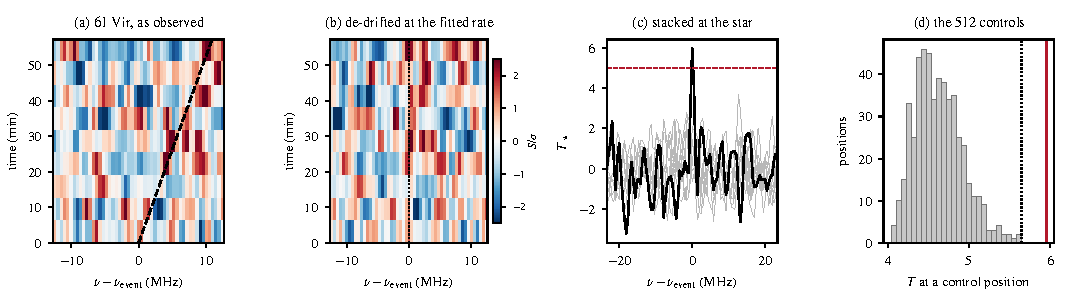
\includegraphics[width=\textwidth]{figures/event_crossings.pdf}
\caption{\textbf{The strongest crossing of the survey, and the control field
it leads.} Frequencies are in the star's rest frame.
\emph{(a)}~The dynamic spectrum at \EvAStar's position around the crossing at
\RqFreqSx\,GHz, observed \EvADate, with the fitted drift of
\EvADrift\,Hz\,s$^{-1}$ as the dashed track; the \EvANInt{} integrations are
binned into \EvANBin{} and plotted in units of each bin's noise. At
\EvAFlux$\pm$\EvAFluxErr\,mJy against \EvARmsInt\,mJy per integration the
carrier is \EvAPerIntSig{} standard deviations in any one of them, and exists
only in the coherent stack of all \EvADwellMin{} minutes on source.
\emph{(b)}~The same rows shifted by that drift, which carries the carrier
\EvADriftChan{} channels of \EvAChanwkHz\,kHz across the observation.
\emph{(c)}~The de-drifted stack at the star (black) and at the
\RcNRetCtrl{} control positions with retained dynamic spectra (grey), in
units of its own noise; dashed, the trigger. \emph{(d)}~The same statistic at
each of the \NCtrl{} rank-screen control positions: the star (solid) against
the highest control (dotted). The recurrence test, for this crossing and for
the second one, \EvBStar{} at \RqFreqCp\,GHz, is in
Table~\ref{tab:cand}, which also gives the implied isotropic-equivalent
powers, $\EvAEirp\times10^{\EvAEirpExp}$\,W at \EvADistPc\,pc here and
$\EvBEirp\times10^{\EvBEirpExp}$\,W at \EvBDistPc\,pc there.}
\label{fig:event}
\end{figure*}

\begin{table}
\centering
\caption{\textbf{Can two crossings be one carrier?} Every pair of crossings
toward one star, in two execution blocks, within
\WdHalfKms\,km\,s$^{-1}$ of each other in the star's frame; stars are
identified by position, so the two archival-tail crossings of \TjDeepStar{}
pair with its catalogued ones. $\Delta\nu$ is the stellar-frame offset and
$\dot\nu_1$, $\dot\nu_2$ the drifts fitted independently in the two blocks
and carried into that frame. A transmitter at constant line-of-sight
acceleration would put the pair at
$\Delta\nu=\frac{1}{2}(\dot\nu_1+\dot\nu_2)\Delta t$, and \emph{miss} is how
far it is from that in units of the drift grid's resolution carried over
$\Delta t$; a dash means that resolution exceeds the window searched, so the
comparison has no power. The last column is the verdict under the weaker
criterion of a bounded trajectory inside the same grid and acceleration
ceiling: \emph{no} where one carrier is excluded, \emph{open} where the pair
is not separable, \emph{yes} for the control row. A fitted drift is refined
inside one grid step and may fall beyond the outermost trial, here by
\TjGridOverStep{} of a \TjGridStepHzS\,Hz\,s$^{-1}$ step, so a value above
may exceed the \DriftCeilLo\,nHz default ceiling of \S\ref{sec:method}
although that window's own outermost trial, \TjGridEdgeNHz\,nHz, does not.}
\label{tab:pairs}
\scriptsize
%% GENERATED by pairs_v415.py -- do not hand-edit.
\begin{tabular}{@{}l@{~}l@{\,}r@{\,}r@{\,}r@{\,}r@{\,}r@{~}l@{}}
\hline
Star & blocks & $\Delta t$ & $\dot\nu_1$ & $\dot\nu_2$ & $\Delta\nu$ & miss & one \\
 & & (d) & \multicolumn{2}{c}{(Hz\,s$^{-1}$)} & (MHz) & ($\sigma$) & carrier? \\
\hline
61~Vir & X822/X82f & 3.00 & $+1092$ & $+3221$ & $+755.4$ & 15 & open \\
J1537$-$3319 & X10359/X398 & 123 & $-2000$ & $+2390$ & $+223.5$ & 3.6 & open \\
AU~Mic & X1838/X319 & 310 & $+1440$ & $+2645$ & $-159.0$ & --- & open \\
HD~14055 & X2b2ee/X2c3bb & 0.09 & $-2390$ & $+4216$ & $+825.2$ & 2447 & no \\
 & X24be0/Xd46 & 1.92 & $+1134$ & $-3823$ & $+63.0$ & 41 & open \\
 & X2c3bb/X3835 & 2.00 & $+4216$ & $+1800$ & $-514.6$ & 144 & no \\
 & X2b2ee/X3835 & 2.09 & $-2390$ & $+1800$ & $+310.6$ & 48 & open \\
 & X3835/Xd526 & 607 & $+1800$ & $-2563$ & $-555.5$ & --- & open \\
 & X2b2ee/Xd526 & 609 & $-2390$ & $-2563$ & $-244.9$ & --- & open \\
 & X3835/X25c5e & 649 & $+1800$ & $+2611$ & $+423.3$ & --- & open \\
 & X2c3bb/X25c5e & 651 & $+4216$ & $+2611$ & $-91.3$ & --- & open \\
 & X2b2ee/X25c5e & 651 & $-2390$ & $+2611$ & $+733.8$ & --- & open \\
$\beta$~Pic & X3a90/Xa9df & 1.02 & $-1611$ & $-679$ & $+85.5$ & 132 & no \\
\hline
HD~285968 & X108f/X5b4e & 4.99 & $-29$ & $-29$ & $-0.002$ & 0.6 & yes \\
\hline
\end{tabular}

\end{table}

\begin{table}
\centering
\caption{\textbf{The two events}, the crossings whose
stellar statistic exceeds all \NCtrl{} control positions of their own window;
the first of them is Fig.~\ref{fig:event}.
Repeat epochs measured are the blocks at which the predicted stellar-frame
cell was read, the remainder of them coming from the archival extension.
$T_{\rm pers}$ is what a carrier persisting at the discovery amplitude $S$
would have given there and $T_{\rm rep}$ is what is measured, combining every
repeat epoch by inverse variance at the carried drift: one cell and one
trial, so it may be negative, while the two indented readings beneath it are
maxima and so positive on average whatever is there. The nearest block alone
follows, because the combination requires the carrier to return to that cell
at the start of every block across the whole baseline and the single reading
requires only the two observations. The exclusion is the fraction of $S$ still
ruled out at the trigger, $(T_{\rm rep}+5)/T_{\rm pers}$; the displacement
permitted is half a channel in the star's frame. The last row but one is the
chance $\Phi(5T_{\rm pers}/T_\star-5)$ that a carrier at the trigger
amplitude $5S/T_\star$ would have satisfied the criterion, and in brackets the
same at $S$, which is selected as the largest of many cells and biased high.}
\label{tab:cand}
\footnotesize
%% GENERATED by recur_v411.py -- do not hand-edit.
\begin{tabular}{@{}>{\raggedright\arraybackslash}p{0.49\columnwidth}@{~~}r@{~~}r@{}}
\hline
 & 61 Vir & CP$-$72 2713 \\
\hline
Frequency, stellar frame (GHz) & 346.323236 & 344.296455 \\
\quad as delivered, topocentric & 346.313811 & 344.269746 \\
Drift rate (Hz\,s$^{-1}$) & $+3182$ & $-2056$ \\
$T_\star$ & 5.958 & 5.809 \\
Highest control $T$ & 5.65 & 5.68 \\
Fitted amplitude (mJy) & 118.8 $\pm$ 19.9 & 11.3 $\pm$ 2.0 \\
Peak-channel EIRP (W) & $5.1 \times 10^{14}$ & $8.9 \times 10^{14}$ \\
Repeat epochs measured & 3 & 5 \\
\quad of them in the primary census & 3 & 1 \\
\quad census repeats with no retained spectrum & 1 & 0 \\
Nearest covering epoch, separation (h) & $-1.97$ & $+2.05$ \\
\quad covering epochs more than a day away & 2 & 4 \\
Longest baseline (d) & 3 & 2 \\
$T$ expected if persistent, $T_{\rm pers}$ & 9.70 & 6.30 \\
$T$ measured, matched drift, $T_{\rm rep}$ & $+0.39$ & $-0.82$ \\
\quad largest single epoch & $+1.65$ & $+0.96$ \\
\quad maximised over every drift & 2.71 & 3.60 \\
Nearest block alone, $T_{\rm pers}$ & 5.28 & 6.21 \\
\quad $T_{\rm rep}$ & $-0.01$ & $-0.57$ \\
Amplitude still excluded, $(T_{\rm rep}+5)/T_{\rm pers}$ & 0.56 $S$ & 0.66 $S$ \\
\quad from the nearest block alone & 0.95 $S$ & 0.71 $S$ \\
Displacement permitted (km\,s$^{-1}$) & $\pm$0.211 & $\pm$0.213 \\
\quad a transmitter at 1\,au would move & 0.042 & 0.044 \\
\quad and over the longest baseline & 1.53 & 1.08 \\
Recovery chance at $5S/T_\star$ (at $S$) & 1.00 (1.00) & 0.66 (0.90) \\
Disposition & not confirmed & not confirmed \\
\hline
\end{tabular}

\end{table}

\begin{table*}
\centering
\caption{\textbf{The threshold crossings of the reserved hold-out}, searched
with the same frozen pipeline and disposed of by the same tests as the
census. $\Delta v_\star$ is the offset from the nearest masked transition in
the star's own frame and $n_{\rm rep}$ the number of covering repeat blocks;
$T_{\rm pers}$ and $T_{\rm rep}$ are as in Table~\ref{tab:ledger}. The one
crossing that is present again is a carbon monoxide line.}
\label{tab:holdout}
\scriptsize
%% GENERATED by holdout_v412.py -- do not hand-edit.
\begin{tabular}{@{}l@{~}l@{~}r@{~}r@{~}l@{~}r@{~~}r@{~}r@{~}r@{~}l@{}}
\hline
Star & block & $\nu_{\rm topo}$ (GHz) & $T_\star$ & line & $\Delta v_\star$ & $n_{\rm rep}$ & $T_{\rm pers}$ & $T_{\rm rep}$ & disposition \\
\hline
HD~285968 & Xdaef5a\_Xdd9b & 230.5081 & 8.642 & CO($2$--$1$) & +8.7 & 4 & 11.6 & +6.71 & attributed; present again \\
HD~14055 & X107376c\_X6126 & 330.7123 & 5.513 & $^{13}$CO($3$--$2$) & +112.6 & 30 & 312.0 & +0.56 & unattributed; does not recur \\
TRAPPIST$-$1 & Xd0e450\_X259b & 346.2454 & 5.326 & SO($9_{8}$--$8_{7}$) & -306.6 & 5 & 11.1 & -0.32 & unattributed; does not recur \\
HD~172555 & X107fa96\_X1300f & 344.6066 & 5.144 & SO($8_{8}$--$7_{7}$) & +251.3 & --- & --- & --- & unattributed; no repeat coverage \\
HD~285968 & Xdb4b9a\_Xa7c & 229.9129 & 5.106 & CO($2$--$1$) & -768.0 & 4 & 11.2 & +0.21 & unattributed; does not recur \\
HR~1010 & Xc6b674\_X23f2 & 346.2301 & 5.044 & SO($9_{8}$--$8_{7}$) & -238.7 & 7 & 25.9 & -0.80 & unattributed; does not recur \\
HD~10647 & Xff99e1\_X9cdf & 345.7059 & 5.017 & SO($2_{3}$--$2_{1}$) & +37.1 & 13 & 142.1 & -0.93 & unattributed; does not recur \\
HD~170773 & Xff294f\_X1fb & 345.5597 & 5.001 & SO($2_{3}$--$2_{1}$) & -113.8 & 4 & 59.3 & +1.45 & unattributed; does not recur \\
\hline
\end{tabular}

\end{table*}

%% tab:ledger MOVED to Appendix D (sections/app_J_falsealarm.tex): a
%% full-width 56-row table* worth 0.72 pp of the main text.  Sec. 5.3 and
%% Sec. 5.6 carry the counts and cite it.



%% fig:chain MOVED to sections/04_method.tex, Sec. 4.2, where it is first
%% cited (referee 2, minor 3).  Sec. 5 cites it at the crossing census.

%% ---------------------------------------------------------------------
%% REQUEST (results owner -> numbers owner).  Eight macros this file uses
%% that the frozen layer does not yet define, all on the adopted
%% trigger-plus-spatial-screen criterion (EirpNinetyMultA = 5.70):
%%   \EirpNinetyWinMedA                      median Class A window, W
%%   \EirpNinetySysLoA \EirpNinetySysMedA \EirpNinetySysHiA
%%                                           per system, best window, W
%%   \EirpNinetyBarnLo \EirpNinetyBarnHi     Barnard's Star, W
%%   \EirpNinetyWolfLo \EirpNinetyWolfHi     Wolf 359, W
%% The \Promote* family (\PromoteMedA, \PromoteSysMedA, ...) is the same
%% quantity on the superseded localisation criterion and is cited nowhere
%% in this file; it is still cited in 03_sample.tex and 07_conclusions.tex,
%% which must move to the names above or the paper will carry two
%% sensitivities again.  \EirpBarnLo/\EirpBarnHi/\EirpWolfLo/\EirpWolfHi
%% are nominal triggers and are no longer quoted here.
%%
%% REQUEST (results owner -> numbers owner).  tab_ledger_v403 must drop
%% nine columns: both visibility-fit epoch groups (Re/sigma, Im/sigma,
%% ctrl, twice), the epoch displacement D, the off-channel column "off",
%% and the "scr" rank flag, whose result is carried by the disposition
%% code.  Eight columns remain: star, block, band, nu, T_star, line, dv,
%% disposition.  \LedgerLegend is replaced by the caption above, so the
%% legend macro is no longer referenced.
%%
%% REQUEST (results owner -> numbers owner).  tab_maskladder.tex now has a
%% home as Table tab:maskladder in this file.  Its fourth column header
%% reads "rank-flagged", a phrase this manuscript has used in both senses;
%% please rename it to "outrank all controls" so the header cannot be read
%% as its own opposite.  The caption states the meaning meanwhile.
%%
%% REQUEST (results owner -> figures owner).  fig:chain MUST BE RE-EMITTED
%% AT SINGLE-COLUMN GEOMETRY.  It is now a \begin{figure} at \columnwidth,
%% not a figure* at 0.98\textwidth, because the section measures 6.0 pp as
%% three full-width floats and 5.0 pp with this one in a column -- the
%% overage was float packing, not words.  chain_v403.pdf is still drawn for
%% full width, so its labels are currently at about half their intended
%% size: PLEASE RE-EMIT FOR ONE COLUMN.  A six-step vertical chain reads
%% better in a column than across a page, so this is the right geometry
%% for it, but the caption, the placement and the artwork must agree and
%% today only two of the three do.  If re-emission is refused, revert this
%% float to figure*/0.98\textwidth and the section is 6.0 pp.
%%
%% REQUEST (results owner -> figures owner).  fig:bpiccontrol.
%%  - GEOMETRY CONFIRMED SINGLE COLUMN.  bpic_control.pdf is 237.6 x 280.7 pt,
%%    i.e. one column wide with the two panels stacked vertically, and the
%%    float is \columnwidth in a \begin{figure}.  Caption and placement
%%    agree; no re-emission at full width is wanted.  Panel (b) gets the
%%    full column width this way, which is what it needs.
%%  - COUNTS I WOULD NOT INVENT.  \NStageOneBpicEb (9) counts the blocks in
%%    which the star outranks every control, so it cannot also count the
%%    points drawn: the ring-wins block is by definition not one of the 9.
%%    The caption therefore says "the 9 ... and one further block" rather
%%    than giving a total.  Four macros would let it say what is drawn:
%%      \BpicPanelNCo     beta Pic CO points in panel (b)        (10)
%%      \BpicPanelNOther  other crossings drawn in grey          (39)
%%      \BpicDvCoLo \BpicDvCoHi   |dv| range of the CO crossings (12-29)
%%      \BpicDvCsLo \BpicDvCsHi   |dv| of the two CS(5-4) crossings
%%    \BpicDvLo/\BpicDvHi existed earlier today and have since been retired.
%%  - COUNTEREXAMPLE NUMBERS, requested and still absent: the ring maximum
%%    (14.13), the stellar statistic (9.68) and the number of the \NCtrl
%%    controls above the star (6) in the ring-wins block.  When they exist
%%    the caption should name that block instead of gesturing at it.
%%
%% REQUEST (results owner -> integrator).  Labels and floats deleted from
%% this file, with the files that still reference them:
%%   sec:linecost     -> sec:bpicval   (06_discussion, app_F, app_I, app_K)
%%   sec:repairedstat -> app:v409      (08_backmatter, app_A, app_M)
%%   eq:tunif         no longer defined anywhere (app_L cites it)
%%   tab:crossdelta   float deleted with the revision-history material;
%%                    app_M_repaired.tex still cites it
%%   tab:clustv409    float deleted; nothing else cites it
%%   fig:ledgervis    no longer cited (float lives in app_K)
%%   tab:hosts        no longer cited from here
%%   app:etacrvrecur  no longer cited from here (app_M still cites it)
%% ---------------------------------------------------------------------
